% Options for packages loaded elsewhere
\PassOptionsToPackage{unicode}{hyperref}
\PassOptionsToPackage{hyphens}{url}
%
\documentclass[
  11pt,
]{article}
\usepackage{amsmath,amssymb}
\usepackage{lmodern}
\usepackage{ifxetex,ifluatex}
\ifnum 0\ifxetex 1\fi\ifluatex 1\fi=0 % if pdftex
  \usepackage[T1]{fontenc}
  \usepackage[utf8]{inputenc}
  \usepackage{textcomp} % provide euro and other symbols
\else % if luatex or xetex
  \usepackage{unicode-math}
  \defaultfontfeatures{Scale=MatchLowercase}
  \defaultfontfeatures[\rmfamily]{Ligatures=TeX,Scale=1}
\fi
% Use upquote if available, for straight quotes in verbatim environments
\IfFileExists{upquote.sty}{\usepackage{upquote}}{}
\IfFileExists{microtype.sty}{% use microtype if available
  \usepackage[]{microtype}
  \UseMicrotypeSet[protrusion]{basicmath} % disable protrusion for tt fonts
}{}
\makeatletter
\@ifundefined{KOMAClassName}{% if non-KOMA class
  \IfFileExists{parskip.sty}{%
    \usepackage{parskip}
  }{% else
    \setlength{\parindent}{0pt}
    \setlength{\parskip}{6pt plus 2pt minus 1pt}}
}{% if KOMA class
  \KOMAoptions{parskip=half}}
\makeatother
\usepackage{xcolor}
\IfFileExists{xurl.sty}{\usepackage{xurl}}{} % add URL line breaks if available
\IfFileExists{bookmark.sty}{\usepackage{bookmark}}{\usepackage{hyperref}}
\hypersetup{
  hidelinks,
  pdfcreator={LaTeX via pandoc}}
\urlstyle{same} % disable monospaced font for URLs
\usepackage[margin=3cm]{geometry}
\usepackage{color}
\usepackage{fancyvrb}
\newcommand{\VerbBar}{|}
\newcommand{\VERB}{\Verb[commandchars=\\\{\}]}
\DefineVerbatimEnvironment{Highlighting}{Verbatim}{commandchars=\\\{\}}
% Add ',fontsize=\small' for more characters per line
\usepackage{framed}
\definecolor{shadecolor}{RGB}{248,248,248}
\newenvironment{Shaded}{\begin{snugshade}}{\end{snugshade}}
\newcommand{\AlertTok}[1]{\textcolor[rgb]{0.94,0.16,0.16}{#1}}
\newcommand{\AnnotationTok}[1]{\textcolor[rgb]{0.56,0.35,0.01}{\textbf{\textit{#1}}}}
\newcommand{\AttributeTok}[1]{\textcolor[rgb]{0.77,0.63,0.00}{#1}}
\newcommand{\BaseNTok}[1]{\textcolor[rgb]{0.00,0.00,0.81}{#1}}
\newcommand{\BuiltInTok}[1]{#1}
\newcommand{\CharTok}[1]{\textcolor[rgb]{0.31,0.60,0.02}{#1}}
\newcommand{\CommentTok}[1]{\textcolor[rgb]{0.56,0.35,0.01}{\textit{#1}}}
\newcommand{\CommentVarTok}[1]{\textcolor[rgb]{0.56,0.35,0.01}{\textbf{\textit{#1}}}}
\newcommand{\ConstantTok}[1]{\textcolor[rgb]{0.00,0.00,0.00}{#1}}
\newcommand{\ControlFlowTok}[1]{\textcolor[rgb]{0.13,0.29,0.53}{\textbf{#1}}}
\newcommand{\DataTypeTok}[1]{\textcolor[rgb]{0.13,0.29,0.53}{#1}}
\newcommand{\DecValTok}[1]{\textcolor[rgb]{0.00,0.00,0.81}{#1}}
\newcommand{\DocumentationTok}[1]{\textcolor[rgb]{0.56,0.35,0.01}{\textbf{\textit{#1}}}}
\newcommand{\ErrorTok}[1]{\textcolor[rgb]{0.64,0.00,0.00}{\textbf{#1}}}
\newcommand{\ExtensionTok}[1]{#1}
\newcommand{\FloatTok}[1]{\textcolor[rgb]{0.00,0.00,0.81}{#1}}
\newcommand{\FunctionTok}[1]{\textcolor[rgb]{0.00,0.00,0.00}{#1}}
\newcommand{\ImportTok}[1]{#1}
\newcommand{\InformationTok}[1]{\textcolor[rgb]{0.56,0.35,0.01}{\textbf{\textit{#1}}}}
\newcommand{\KeywordTok}[1]{\textcolor[rgb]{0.13,0.29,0.53}{\textbf{#1}}}
\newcommand{\NormalTok}[1]{#1}
\newcommand{\OperatorTok}[1]{\textcolor[rgb]{0.81,0.36,0.00}{\textbf{#1}}}
\newcommand{\OtherTok}[1]{\textcolor[rgb]{0.56,0.35,0.01}{#1}}
\newcommand{\PreprocessorTok}[1]{\textcolor[rgb]{0.56,0.35,0.01}{\textit{#1}}}
\newcommand{\RegionMarkerTok}[1]{#1}
\newcommand{\SpecialCharTok}[1]{\textcolor[rgb]{0.00,0.00,0.00}{#1}}
\newcommand{\SpecialStringTok}[1]{\textcolor[rgb]{0.31,0.60,0.02}{#1}}
\newcommand{\StringTok}[1]{\textcolor[rgb]{0.31,0.60,0.02}{#1}}
\newcommand{\VariableTok}[1]{\textcolor[rgb]{0.00,0.00,0.00}{#1}}
\newcommand{\VerbatimStringTok}[1]{\textcolor[rgb]{0.31,0.60,0.02}{#1}}
\newcommand{\WarningTok}[1]{\textcolor[rgb]{0.56,0.35,0.01}{\textbf{\textit{#1}}}}
\usepackage{graphicx}
\makeatletter
\def\maxwidth{\ifdim\Gin@nat@width>\linewidth\linewidth\else\Gin@nat@width\fi}
\def\maxheight{\ifdim\Gin@nat@height>\textheight\textheight\else\Gin@nat@height\fi}
\makeatother
% Scale images if necessary, so that they will not overflow the page
% margins by default, and it is still possible to overwrite the defaults
% using explicit options in \includegraphics[width, height, ...]{}
\setkeys{Gin}{width=\maxwidth,height=\maxheight,keepaspectratio}
% Set default figure placement to htbp
\makeatletter
\def\fps@figure{htbp}
\makeatother
\setlength{\emergencystretch}{3em} % prevent overfull lines
\providecommand{\tightlist}{%
  \setlength{\itemsep}{0pt}\setlength{\parskip}{0pt}}
\setcounter{secnumdepth}{-\maxdimen} % remove section numbering
\newcommand*{\secref}[1]{Section~\ref{#1}}
\usepackage{xcolor,colortbl}
\definecolor{gray1}{gray}{0.9}
\ifluatex
  \usepackage{selnolig}  % disable illegal ligatures
\fi

\author{}
\date{\vspace{-2.5em}}

\begin{document}

\hypertarget{practical-part---colorectal-cancer}{%
\section{2.1 Practical part - Colorectal
Cancer}\label{practical-part---colorectal-cancer}}

\hypertarget{show-if-covariates-are-important-for-death-using-cox-modelling.-estimate-the-survival-distribution-for-relevant-covariate-combinations.}{%
\subsection{1. Show if covariates are important for death using Cox
modelling. Estimate the survival distribution for relevant covariate
combinations.}\label{show-if-covariates-are-important-for-death-using-cox-modelling.-estimate-the-survival-distribution-for-relevant-covariate-combinations.}}

First, we note that the data given consists of a subset containing 150
patients of the original randomized trial including 410 patients. We
assume that this is a randomly chosen subset such that the randomization
is still valid (this is a plausible assumption according to
help(colorectal)). The time variables are reported in years, so we
choose to multiply with 12 to obtain a time scale of months instead.

In this and the following question, we consider the terminal event death
as the event of interest. First, we fit a cox model using the covariates
treatment, age and who.ps (WHO performance status at baseline), and
ignore the number of new lesions for now:

\begin{Shaded}
\begin{Highlighting}[]
\NormalTok{colo.sub }\OtherTok{\textless{}{-}}\NormalTok{ colo[}\FunctionTok{order}\NormalTok{(id, time1)]}
\NormalTok{colo.sub }\OtherTok{\textless{}{-}}\NormalTok{ colo.sub[,.SD[.N],by}\OtherTok{=}\NormalTok{id] }\CommentTok{\#Only last event (death)}
\NormalTok{m.cox }\OtherTok{\textless{}{-}} \FunctionTok{coxph}\NormalTok{(}\FunctionTok{Surv}\NormalTok{(time1, state)}\SpecialCharTok{\textasciitilde{}}\NormalTok{treatment }\SpecialCharTok{+}\NormalTok{ age }\SpecialCharTok{+}\NormalTok{ who.PS, }\AttributeTok{data =}\NormalTok{ colo.sub)}
\end{Highlighting}
\end{Shaded}

Before interpreting the model results, we need to chech that the
important assumption of proportional hazards is fulfilled, ie. that the
effect of the covariates is constant over time. We do this by
considering the cumulative martingale residuals, and the cumulative
score process test for proportionality. This is done using the gof
(goodness of fit) function. We get:

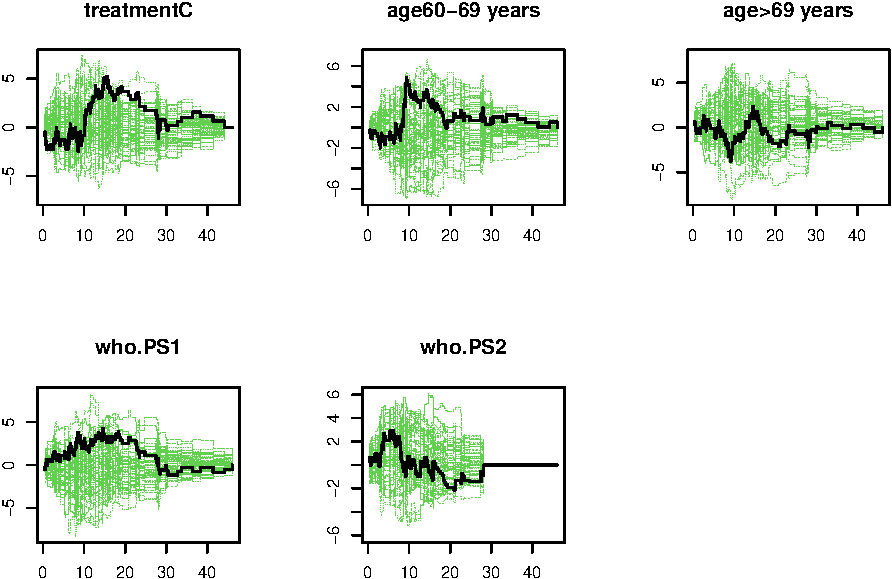
\includegraphics{Exam2021_PracticalPart_files/figure-latex/unnamed-chunk-4-1.pdf}

We see for all covariates, that the black line lies within the green
ones, which indicates that the proportional hazards assumption is
fulfilled. If we consider the goodness of fit object, we get the
cumulative score process test for proportionality:

\begin{verbatim}
## Cumulative score process test for Proportionality:
##                Sup|U(t)|  pval
## treatmentC      5.240899 0.218
## age60-69 years  4.844747 0.232
## age>69 years    3.763129 0.586
## who.PS1         4.217036 0.436
## who.PS2         2.949119 0.641
\end{verbatim}

All the covariates have a non-significant p-value (\(>0.05\)), which
again indicates that the proportional hazards assumption can be assumed.
We therefore continue with the model. Below, the coefficients from the
model are shown:

\begin{Shaded}
\begin{Highlighting}[]
\FunctionTok{summary}\NormalTok{(m.cox)}\SpecialCharTok{$}\NormalTok{coef}
\end{Highlighting}
\end{Shaded}

\begin{verbatim}
##                       coef exp(coef)  se(coef)          z     Pr(>|z|)
## treatmentC     -0.11670324 0.8898492 0.1906453 -0.6121484 0.5404395821
## age60-69 years -0.18286815 0.8328780 0.2347132 -0.7791132 0.4359130173
## age>69 years   -0.22058062 0.8020530 0.2184044 -1.0099641 0.3125125108
## who.PS1        -0.07389633 0.9287680 0.2083767 -0.3546286 0.7228678711
## who.PS2         0.87175235 2.3910972 0.2449886  3.5583388 0.0003732077
\end{verbatim}

Not taking new lesions into account and only considering the effect of
the three covariates on death, we see from the summary that treatment
and age do not seem to affect death significantly (assuming a confidence
level of 5 \(\%\)). However, it seems that the hazard of dying for who
status 2 is significantly higher as compared to status 0 (between 1.44
and 3.82 times higher). This is also seen, when considering the survival
functions below, where it seems that the group with who status 2 in
general has a lower survival probability than the other two groups.
Also, the curves for the different groups of treatment and age are
overlapping, which indicate no effect on death of these covariates.

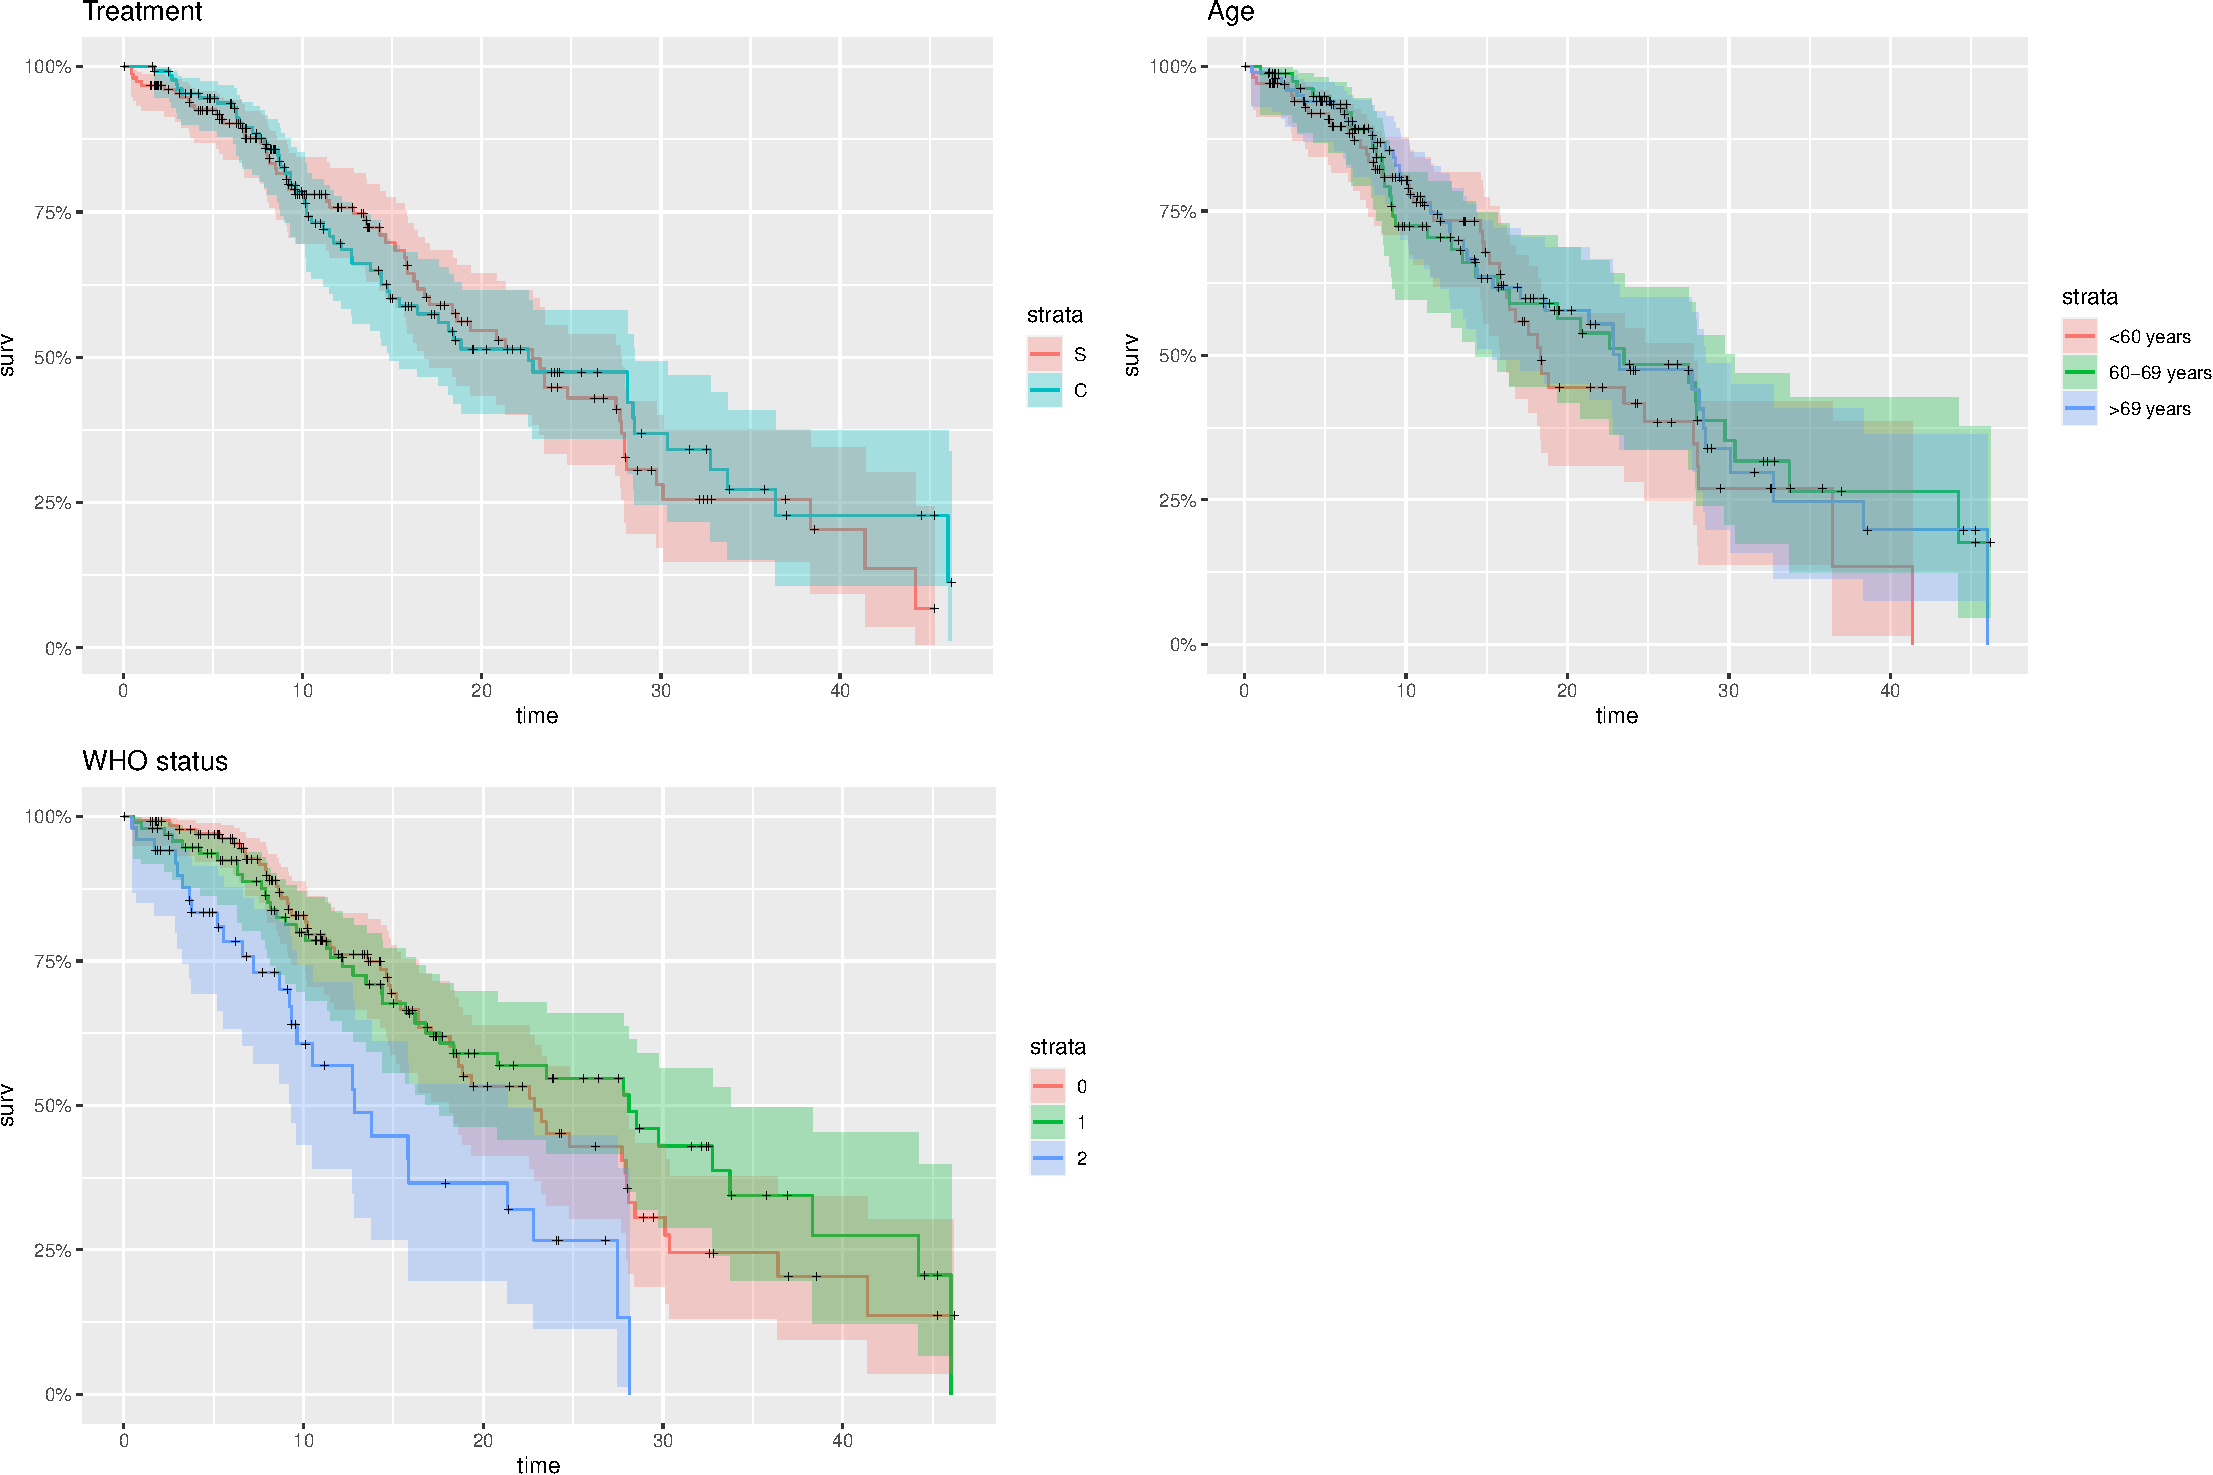
\includegraphics{Exam2021_PracticalPart_files/figure-latex/unnamed-chunk-7-1.pdf}

We now consider the survival function for chosen combinations of
covariates. First, we take a look at treatment and the who status:

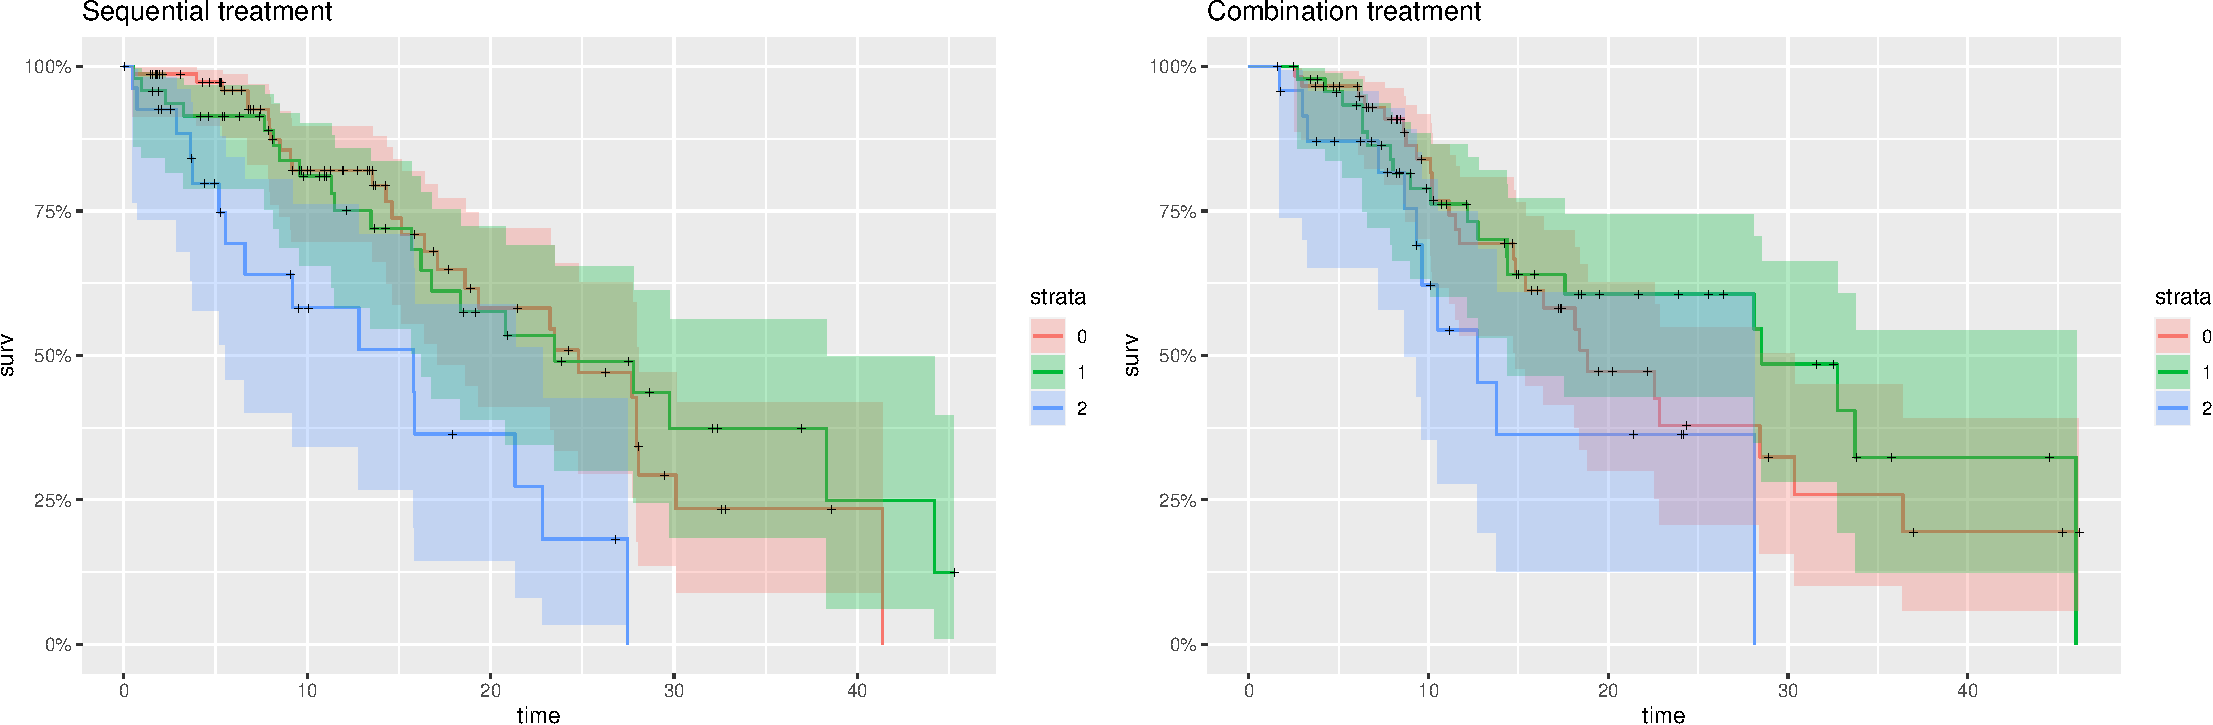
\includegraphics{Exam2021_PracticalPart_files/figure-latex/unnamed-chunk-8-1.pdf}

When stratifying by treatment, we see that the difference in survival on
the who groups is mostly driven by the sequential treatment group, where
the curve for strata 2 is lower at all times. The survival curve for who
status 2 for combination treatment is also lower than the other two at
some time points, but at other time points, the curves are crossing. A
general picture when stratifying by treatment is that who group 0 and 1
are more similar as compared to group 2, which the cox model and the
overall summary also indicated.

We now consider a combination of treatment and age:

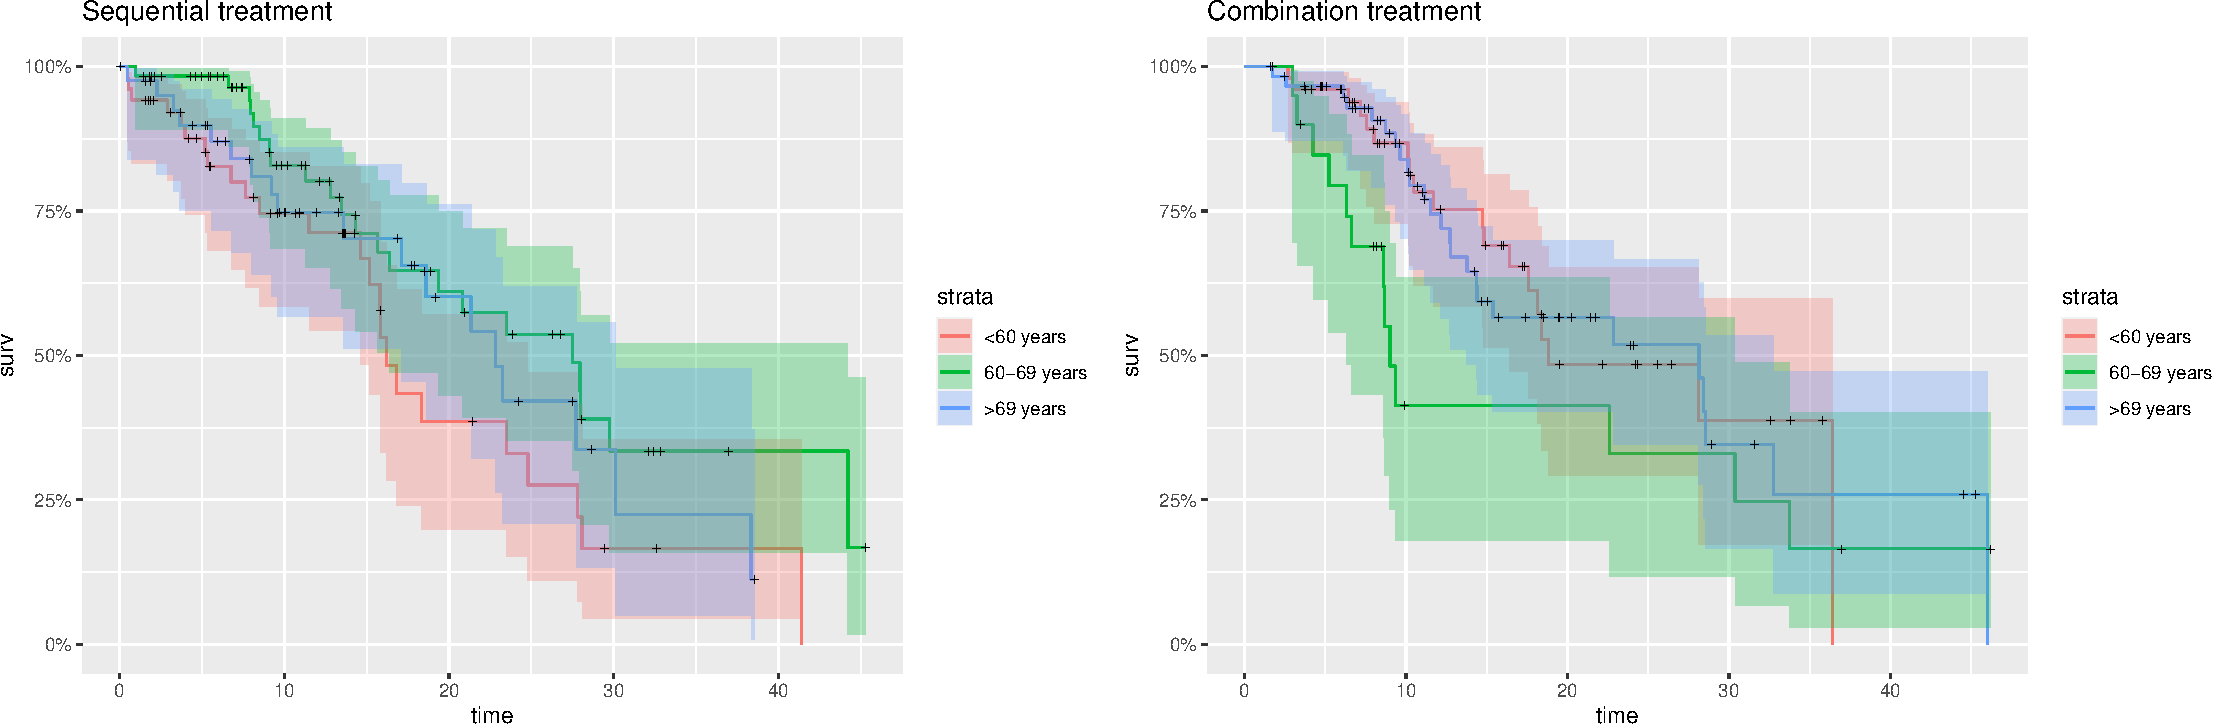
\includegraphics{Exam2021_PracticalPart_files/figure-latex/unnamed-chunk-9-1.pdf}

For the sequential treatment, the survival curves are overlapping,
however, the combination treatment seems to be working more poorly for
people aged 60-69, especially during the first 10 months. Note however,
that there is only 15 subjects in this subgroup.

\hypertarget{is-death-and-the-number-new-lesions-related}{%
\subsection{2. Is death and the number new lesions
related?}\label{is-death-and-the-number-new-lesions-related}}

To answer this question, we construct a variable, stating the number of
new lesions per person (id), as a cumulated sum per time point. This is
included in the cox model as a factor. Note that in order not to
condition on the future (the end of the time interval when we are at the
beginning of the time interval), we shift the sum of lesions to the next
time interval. This is done in the following way:

\begin{Shaded}
\begin{Highlighting}[]
\NormalTok{colo }\OtherTok{\textless{}{-}}\NormalTok{ colo[}\FunctionTok{order}\NormalTok{(id, time1)]}
\NormalTok{colo[, num.lesions}\SpecialCharTok{:}\ErrorTok{=}\FunctionTok{head}\NormalTok{(}\FunctionTok{c}\NormalTok{(}\DecValTok{0}\NormalTok{,}\FunctionTok{cumsum}\NormalTok{(new.lesions)),}\AttributeTok{n=}\SpecialCharTok{{-}}\DecValTok{1}\NormalTok{), by}\OtherTok{=}\NormalTok{id] }\CommentTok{\#Shift number of lesions}
\end{Highlighting}
\end{Shaded}

We fit a cox model using this as a covariate, with a cluster(id), as we
have repeated measurements per id. We could also have modelled the
repeated measurements per subject with a frailty model, adding
frailty(id), but we choose use the cluster(id), where a robust estimate
of the standard errors is used. Thereby, possible dependence between the
subjects is modelled. As mentioned, this could also have been done with
a frailty model, where the dependence between subjects is modelled
usually as gamma or log-normal random effects. Furthermore, we now
include both time1 as before, as well as time0, which is the start of
the time interval (0 or the previous recurrence time). This is done as
we now have a time-dependent covariate (number of previous lesions).

\begin{Shaded}
\begin{Highlighting}[]
\NormalTok{m.cox}\FloatTok{.1} \OtherTok{\textless{}{-}} \FunctionTok{coxph}\NormalTok{(}\FunctionTok{Surv}\NormalTok{(time0, time1, state) }\SpecialCharTok{\textasciitilde{}}\NormalTok{ treatment }\SpecialCharTok{+}\NormalTok{ age }\SpecialCharTok{+}\NormalTok{ who.PS }\SpecialCharTok{+} 
                   \FunctionTok{factor}\NormalTok{(num.lesions) }\SpecialCharTok{+} \FunctionTok{cluster}\NormalTok{(id), }\AttributeTok{ties =} \StringTok{"breslow"}\NormalTok{, }\AttributeTok{data =}\NormalTok{ colo)}
\FunctionTok{summary}\NormalTok{(m.cox}\FloatTok{.1}\NormalTok{)}\SpecialCharTok{$}\NormalTok{coef[,}\FunctionTok{c}\NormalTok{(}\DecValTok{1}\SpecialCharTok{:}\DecValTok{3}\NormalTok{, }\DecValTok{6}\NormalTok{)]}
\end{Highlighting}
\end{Shaded}

\begin{verbatim}
##                             coef  exp(coef)  se(coef)     Pr(>|z|)
## treatmentC            0.13164623  1.1407047 0.2012575 4.893092e-01
## age60-69 years       -0.07748919  0.9254370 0.2395318 7.375575e-01
## age>69 years         -0.12656520  0.8811167 0.2234081 5.322327e-01
## who.PS1               0.06843643  1.0708326 0.2174377 7.345618e-01
## who.PS2               0.80740339  2.2420786 0.2549318 6.131510e-04
## factor(num.lesions)1  1.04165371  2.8338996 0.2427865 2.034942e-05
## factor(num.lesions)2  1.74143643  5.7055331 0.2941080 3.137937e-10
## factor(num.lesions)3  1.64951228  5.2044409 0.4161579 2.765895e-08
## factor(num.lesions)4  2.81231787 16.6484626 0.8138383 1.842198e-06
\end{verbatim}

From the summary, we can see that the hazard of dying (as compared to no
new lesions) is increasing with the number of new lesions (significant
increase for all lesion groups). The same picture is seen in the
survival curve below. Note that in the four lesion group, there are only
two subjects that both die after around 27 months, which gives this
sudden fall in the survival curve. So, it could seem that subjects with
four lesions have a longer lifespan, but after a certain time threshold,
they die. All the 9 subjects in the three lesion group also die
eventually. From the figure, we can also see that having one and two
lesions affects the hazard of death similarly over time.

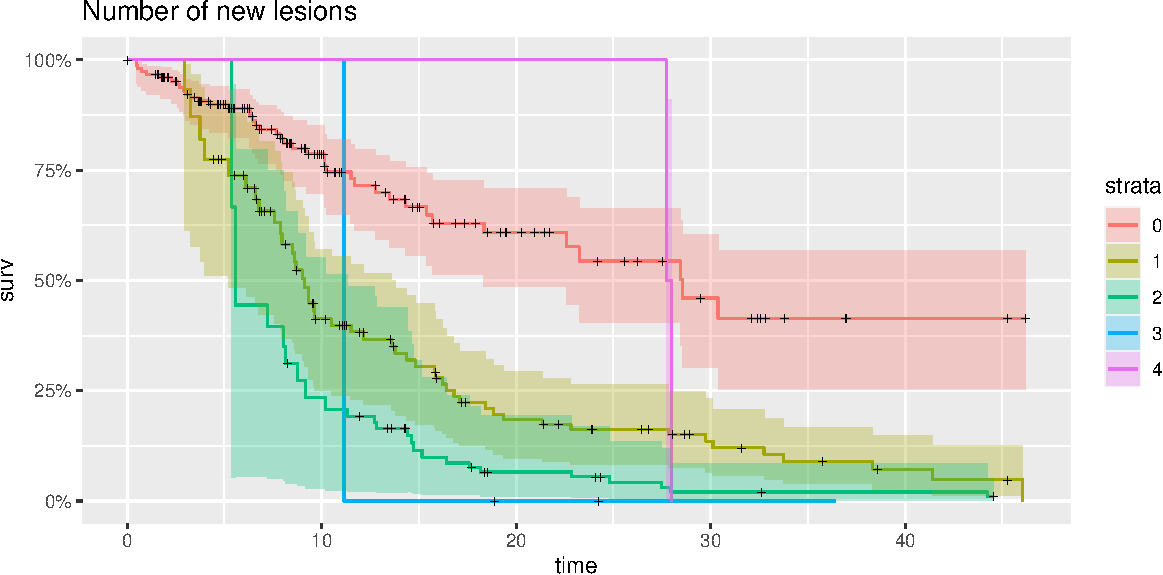
\includegraphics{Exam2021_PracticalPart_files/figure-latex/unnamed-chunk-12-1.pdf}
As we have so few subjects in the four and three lesion group, we try to
model the number of lesions as continous instead. We fit a cox model
using this continous covariate, again with a time0 and cluster(id), as
we have repeated measurements per id:

\begin{Shaded}
\begin{Highlighting}[]
\NormalTok{m.cox}\FloatTok{.2} \OtherTok{\textless{}{-}} \FunctionTok{coxph}\NormalTok{(}\FunctionTok{Surv}\NormalTok{(time0, time1, state) }\SpecialCharTok{\textasciitilde{}}\NormalTok{ treatment }\SpecialCharTok{+}\NormalTok{ age }\SpecialCharTok{+}\NormalTok{ who.PS }\SpecialCharTok{+} 
\NormalTok{                   num.lesions }\SpecialCharTok{+} \FunctionTok{cluster}\NormalTok{(id), }\AttributeTok{data =}\NormalTok{ colo)}
\FunctionTok{summary}\NormalTok{(m.cox}\FloatTok{.2}\NormalTok{)}\SpecialCharTok{$}\NormalTok{coef[,}\FunctionTok{c}\NormalTok{(}\DecValTok{1}\SpecialCharTok{:}\DecValTok{3}\NormalTok{, }\DecValTok{6}\NormalTok{)]}
\end{Highlighting}
\end{Shaded}

\begin{verbatim}
##                       coef exp(coef)  se(coef)     Pr(>|z|)
## treatmentC      0.08024854 1.0835563 0.2001348 6.762475e-01
## age60-69 years -0.05947281 0.9422612 0.2360205 7.972544e-01
## age>69 years   -0.11083703 0.8950846 0.2219450 5.931337e-01
## who.PS1         0.10627110 1.1121233 0.2147533 6.025588e-01
## who.PS2         0.89508456 2.4475427 0.2469690 9.699862e-05
## num.lesions     0.66554204 1.9455448 0.1040912 4.929986e-13
\end{verbatim}

We can see that the hazard of dying increases significantly with number
of lesions which we also expected from the graphical interpretation.

\hypertarget{estimate-the-mean-number-of-new-lessions-as-a-function-of-time-i.e.-the-marginal-mean-of-the-recurrent-events-mut-in-the-previous-exercise.}{%
\subsection{\texorpdfstring{3. Estimate the mean number of new lessions
as a function of time, i.e., the marginal mean of the recurrent events
(\(\mu(t)\) in the previous
exercise).}{3. Estimate the mean number of new lessions as a function of time, i.e., the marginal mean of the recurrent events (\textbackslash mu(t) in the previous exercise).}}\label{estimate-the-mean-number-of-new-lessions-as-a-function-of-time-i.e.-the-marginal-mean-of-the-recurrent-events-mut-in-the-previous-exercise.}}

We now wish to take the re-occurence of new lesions into account, and
estimate the mean number of new lesions as a function of time. Following
Per's slides, we assume that there is no ``gap'' times, ie. a periods
where a new lesion was not possible. It is also a plausible assumption
that a subject is at risk for getting a lesion again immediately after
experiencing a lesion. As we saw in the previous exercise, a large
number of the subjects experience the terminal event death, so we have
presence of a non-negligible mortality rate that we need to take into
account in the modelling.

When mortality plays a role, the Nelson-Aalen estimator for \(\mu(t)\)
will be upwards biased, as events can only happen as long as the subject
is still alive. We will use a simple estimator for \(\mu(t)\) that
accounts for mortality, which is given by the ``Gosh-Lin'' estimator. To
do this in R, we use the phreg function from the mets package. First, we
estimate the mean number of new lesions non-parametrically in the
following way (inlcuding the same covariates as in the previous
exercises, stratifying by treatment as using the cluster(id) option as
argued earlier):

\begin{Shaded}
\begin{Highlighting}[]
\FunctionTok{library}\NormalTok{(mets)}
\NormalTok{survobj }\OtherTok{\textless{}{-}} \FunctionTok{phreg}\NormalTok{(}\FunctionTok{Surv}\NormalTok{(time0, time1, state }\SpecialCharTok{==} \DecValTok{1}\NormalTok{) }\SpecialCharTok{\textasciitilde{}} \FunctionTok{strata}\NormalTok{(treatment) }\SpecialCharTok{+}\NormalTok{ age }\SpecialCharTok{+} 
\NormalTok{                   who.PS }\SpecialCharTok{+} \FunctionTok{cluster}\NormalTok{(id), }\AttributeTok{data =}\NormalTok{ colo, }\AttributeTok{km =} \ConstantTok{TRUE}\NormalTok{)}
\NormalTok{recevobj }\OtherTok{\textless{}{-}} \FunctionTok{phreg}\NormalTok{(}\FunctionTok{Surv}\NormalTok{(time0, time1, new.lesions }\SpecialCharTok{==} \DecValTok{1}\NormalTok{) }\SpecialCharTok{\textasciitilde{}} \FunctionTok{strata}\NormalTok{(treatment) }\SpecialCharTok{+} 
\NormalTok{                  age }\SpecialCharTok{+}\NormalTok{ who.PS }\SpecialCharTok{+} \FunctionTok{cluster}\NormalTok{(id), }\AttributeTok{data =}\NormalTok{ colo, }\AttributeTok{km =} \ConstantTok{TRUE}\NormalTok{)}

\NormalTok{obj }\OtherTok{\textless{}{-}} \FunctionTok{recmarg}\NormalTok{(recevobj, survobj)}
\FunctionTok{bplot}\NormalTok{(obj, }\AttributeTok{ylab =} \StringTok{"Mean number of lesions"}\NormalTok{)}
\end{Highlighting}
\end{Shaded}

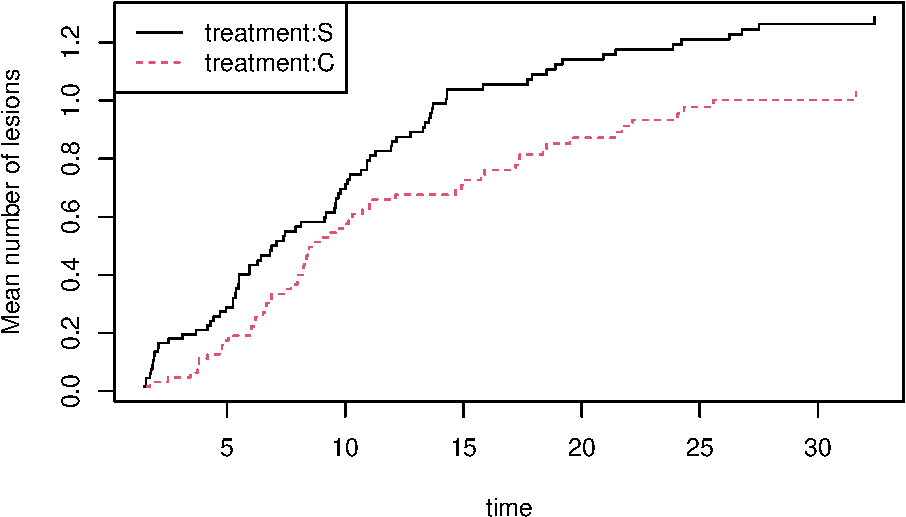
\includegraphics{Exam2021_PracticalPart_files/figure-latex/unnamed-chunk-14-1.pdf}

This shows, that over time, the mean number of lesions is larger for
sequential than combination treatment. The effect seems roughly constant
over time (one might argue that the effect is more pronounced after
around 12 months, but the effect is not noticeable from the plot). We
now estimate the treatment effect on the mean function in a Ghosh-Lin
regression model using the recreg function in the mets package. Note
that to do this, we need to construct a censoring variable, and we also
construct the variable ``status'', which contains information about both
death and lesions, such that:

\begin{itemize}
\tightlist
\item
  status=0 means alive and no lesion
\item
  status=1 means dead
\item
  status=2 means alive and new lesion.
\end{itemize}

\begin{Shaded}
\begin{Highlighting}[]
\NormalTok{colo[,status}\SpecialCharTok{:}\ErrorTok{=}\NormalTok{state]}
\NormalTok{colo[new.lesions}\SpecialCharTok{==}\DecValTok{1}\NormalTok{,status}\SpecialCharTok{:}\ErrorTok{=}\DecValTok{2}\NormalTok{]}
\NormalTok{colo}\SpecialCharTok{$}\NormalTok{cens }\OtherTok{\textless{}{-}}\FunctionTok{ifelse}\NormalTok{(colo}\SpecialCharTok{$}\NormalTok{state}\SpecialCharTok{==}\DecValTok{0}\NormalTok{,}\DecValTok{1}\NormalTok{,}\DecValTok{0}\NormalTok{) }\CommentTok{\#Censoring variable}
\NormalTok{m.goshlin }\OtherTok{\textless{}{-}} \FunctionTok{recreg}\NormalTok{(}\FunctionTok{EventCens}\NormalTok{(time0, time1, status, cens) }\SpecialCharTok{\textasciitilde{}}\NormalTok{ treatment }\SpecialCharTok{+}\NormalTok{ age }\SpecialCharTok{+}\NormalTok{ who.PS }\SpecialCharTok{+} 
                    \FunctionTok{cluster}\NormalTok{(id), }\AttributeTok{data =}\NormalTok{ colo, }\AttributeTok{cause =} \DecValTok{2}\NormalTok{, }\AttributeTok{death.code =} \DecValTok{1}\NormalTok{, }
                    \AttributeTok{cens.code =} \DecValTok{1}\NormalTok{, cens.model }\SpecialCharTok{\textasciitilde{}} \DecValTok{1}\NormalTok{)}
\FunctionTok{summary}\NormalTok{(m.goshlin)}\SpecialCharTok{$}\NormalTok{coef}
\end{Highlighting}
\end{Shaded}

\begin{verbatim}
##                   Estimate      S.E.   dU^-1/2   P-value
## treatmentC     -0.25053314 0.1592898 0.1758116 0.1157620
## age60-69 years -0.12319697 0.1902138 0.2126833 0.5171944
## age>69 years   -0.13647908 0.1863036 0.2025636 0.4638252
## who.PS1        -0.23099135 0.1792848 0.1929288 0.1976052
## who.PS2        -0.04935763 0.2019346 0.2369963 0.8069026
\end{verbatim}

The model is fitted using the same covariates as in the previous
exercises. As expected from the plot above, the mean number of lesions
is lower over time for combination treatment, with an estimated mean
ratio of \(\exp(-0.25053314)=0.78\). This means that, constant over
time, we have \(22\%\) less lesions for combination as compared to
sequential treatment. Note, however, that the treatment effect is
non-significant, with a p-value of \(0.11 > 0.05\).

\hypertarget{estimate-the-probability-of-a-patient-having-more-than-one-new-lesion-before-dying-as-a-function-of-time.}{%
\subsection{4. Estimate the probability of a patient having more than
one new lesion before dying as a function of
time.}\label{estimate-the-probability-of-a-patient-having-more-than-one-new-lesion-before-dying-as-a-function-of-time.}}

In the previous exercise, we considered the mean number of new lesions,
however, now we wish to investigate another summary measure, namely the
probability of a patient having more than one new lesion. For this
purpose, we use the function prob.exceedRecurrent from the mets package
(\url{https://cran.r-project.org/web/packages/mets/vignettes/recurrent-events.html}):

\begin{Shaded}
\begin{Highlighting}[]
\NormalTok{prob.obj }\OtherTok{\textless{}{-}} \FunctionTok{count.history}\NormalTok{(colo, }\AttributeTok{status=}\StringTok{"new.lesions"}\NormalTok{) }\CommentTok{\#Set up data}
\NormalTok{prob.exceed }\OtherTok{\textless{}{-}} \FunctionTok{prob.exceedRecurrent}\NormalTok{(prob.obj, }\DecValTok{1}\NormalTok{, }\AttributeTok{status =} \StringTok{"new.lesions"}\NormalTok{, }
                                    \AttributeTok{death=}\StringTok{"state"}\NormalTok{, }\AttributeTok{start=}\StringTok{"time0"}\NormalTok{, }\AttributeTok{stop=}\StringTok{"time1"}\NormalTok{, }\AttributeTok{id=}\StringTok{"id"}\NormalTok{)}
\FunctionTok{bplot}\NormalTok{(prob.exceed, }\AttributeTok{ylab=}\StringTok{"Probability of exceeding number of lesions"}\NormalTok{)}
\end{Highlighting}
\end{Shaded}

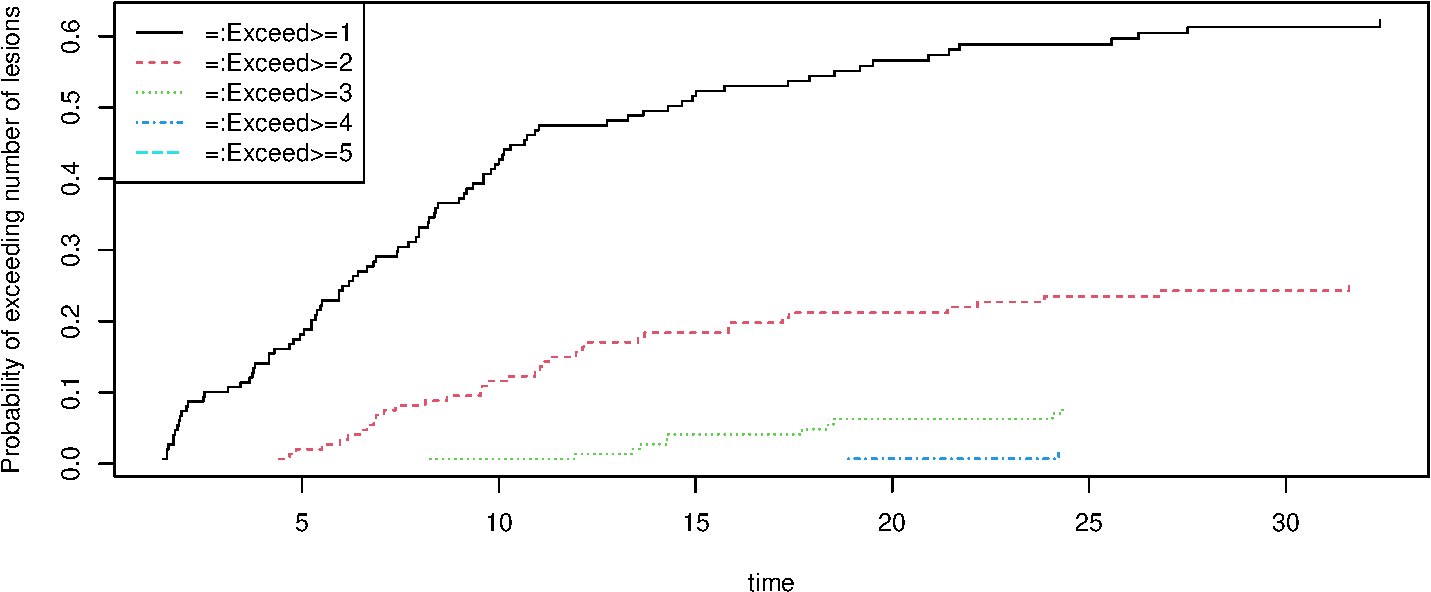
\includegraphics{Exam2021_PracticalPart_files/figure-latex/unnamed-chunk-16-1.pdf}

So, the probability we are interested in is getting more than one lesion
(\(>1\)), which is the red curve (two or above). So, not including any
covariates, the probability of getting more than one lesion is
increasing with time (as expected), with a steeper increase in the first
months. For example, after 10 months, the probability of getting more
than one lesion is around \(10 \%\), and after 25 months, it is
approximately \(23 \%\).

\begin{itemize}
\item
  Investigate if covariates are important for this probability by
  fitting an appropriate regression model.
\item
  Remember to check the assumptions and validate the regression model.
\end{itemize}

\hypertarget{estimate-the-probability-of-a-patient-having-more-than-two-new-lessions-before-dying-as-a-function-of-time.}{%
\subsection{5. Estimate the probability of a patient having more than
two new lessions before dying as a function of
time.}\label{estimate-the-probability-of-a-patient-having-more-than-two-new-lessions-before-dying-as-a-function-of-time.}}

\begin{itemize}
\tightlist
\item
  Same procedure as in question 4.
\end{itemize}

\end{document}
